\documentclass[12pt]{article}

\usepackage{fullpage}
\usepackage{hyperref}
\usepackage{graphicx}
\usepackage{color}
\usepackage{enumerate}
\author{Eric Ruleman, Katherine Yu, Catherine Yun}
\begin{document}

\title{6.005 Project 2 Design Document (Revised)}
\begin{titlepage}
\maketitle
\end{titlepage}
\section{Overview/Implementation Choices}


Our implementation of the collaborative whiteboard currently allows users to draw ovals and make freehand marks. We also allow users to undo and redo changes to each whiteboard. Each client has a reference to its own model that stores the state of a given whiteboard, but these models are not shared between clients, or client and the server. They are each altered the same way (given that they all pertain to the same whiteboard) through message passing and a shared edits queue in the server. All edits must be processed by the server before they are populated on a client's canvas, ensuring that no concurrency bugs occur.\\\\
Each whiteboard is identified by a numerical integer ID number. Users can access a specific whiteboard from the whiteboard selection pane upon first entry, or they can switch between whiteboards once they have already
entered a whiteboard. A user can only be on one Whiteboard at a time, and usernames are unique (no duplicates are allowed). 

\section{Snapshot Diagram}
\begin{figure}[ht!]
\centerline{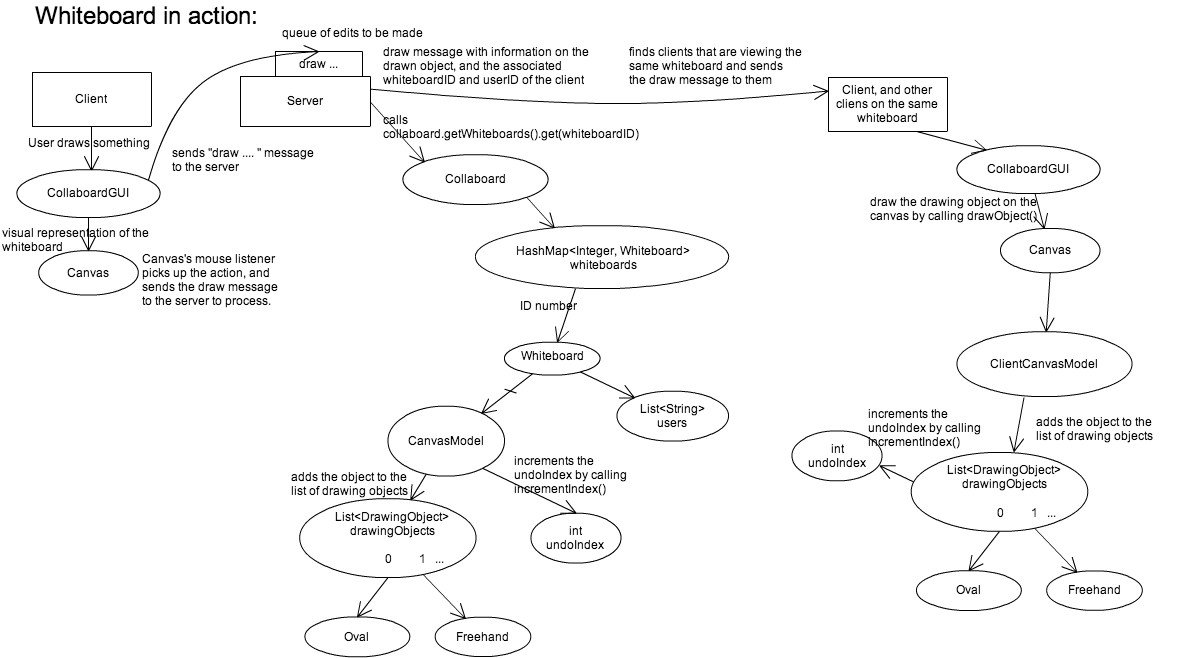
\includegraphics[width=210mm]{snapshot}}
\end{figure}

\section{Datatype Design}
CollaboardServer: Server class for our collaborative whiteboard.
\begin{itemize}
\item Stores the current instance of Collaboard, and current active UserThreads.
\item Handles messages passed from each client thread.
\item Has a BlockingQueue for requests to mutate a whiteboard to be put in and handled one at a time by a thread specifically dedicated to handling requests
\end{itemize}
Collaboard: Class that stores all the active whiteboards and active usernames during a given server session.
\begin{itemize}
\item has a Set of usernames in order to prevent users from creating duplicate usernames
\item has a HashMap of WhiteboardIDs to whiteboards to prevent users from creating whiteboards with duplicate ID numbers
\end{itemize}
Whiteboard: Class representing the state of a given collaborative whiteboard. 
\begin{itemize}
\item  has a CanvasModel
\item  has a list of users currently accessing that whiteboard
\item has a whiteboardID number
\item threadsafe through use of the monitor pattern (will elaborate later in concurrency strategy)
\end{itemize}
CanvasModel: Class representing the state of the canvas in a whiteboard. 
\begin{itemize}
\item  stores an ArrayList of DrawingObjects in the order that they are drawn on the canvas.
\item  stores an undoIndex to determine which objects should be displayed on the canvas
\item  threadsafe through use of the monitor pattern (will elaborate later in concurrency strategy)
\end{itemize}
DrawingObject: An Interface implemented currently by Freehand and Oval. 
\begin{itemize}
\item  Each DrawingObject represents a new stroke or image added to a canvas.
\item  This makes it easy to add new features to our whiteboard, like the ability to draw other shapes like triangles or rectangles.
\item  Freehand: represents a freehand stroke made by a user. Contains a list of Line objects, which store a starting x and y coordinate, an ending x and y coordinate, a string representation of a color, and a string representation of a thickness.
\item  Oval: represents an oval made by a user. Contains a starting x and y coordinate, a center x and y coordinate, a string representation of a color, and a string representation of a thickness.
\end{itemize}
User: Class representing a user currently using the collaborative whiteboard system.
\begin{itemize}
\item  has a userID - unique and assigned by the server upon connection. Used for identification purposes. (Also allows our code to be modified in the case that we allow users to change their usernames without disconnecting.)
\item  has a username: name that is displayed when the user enters a whiteboard. 
\item  has a whiteboardID - ID of the Whiteboard the user is currently accessing.
\item  has a ToolbarModel: Class representing the Color and Thickness settings a given user has active.
\end{itemize}
UserThread: Class representing a client connection on the server.
\begin{itemize}
\item  stores a username, userID, and currentWhiteboardID.
\end{itemize}
Client: Class representing a socket connection to the server. Also handles inputs from the server.
\begin{itemize}
\item  stores a User object
\item  stores a reference to a CollaboardGUI in order to call methods accordingly to mutate the GUI according to inputs from the server.
\item  all of these such calls are made using SwingUtilities.invokeLater() to prevent concurrency issues with Swing.
\end{itemize}
CollaboardGUI: GUI class of the collaborative whiteboard. Populated upon connection to the server.
\begin{itemize}
\item  The first panel the client sees is one in which they select a username. If the username is taken or invalid, an error is displayed. Otherwise, the username is stored client-side and by the server and the user is taken to the next window.
\item  The second panel the client sees is for whiteboard selection. The client can either choose to create a new whiteboard, or select an existing whiteboard from the list of existing whiteboard IDs. 
\item  Once a valid whiteboard is created or selected, the main GUI is shown, consisting of a Canvas, a ToolbarGUI, a JScrollPane displaying active users, and a header that allows the user to switch whiteboards by inputting a new whiteboardID.
\item  ToolbarGUI: Has buttons that the users can toggle to select a drawing color and thickness of the user's ToolbarModel, as well as undo and redo changes to the Canvas. 
\item  has a ClientCanvasModel (in the Canvas) - each client has its version of the CanvasModel stored by the server.
\end{itemize}
\section{Protocol}
From the Server to the Client:
\begin{itemize}
     \item \textbf {VALIDUSER} Allows the client to proceed to the whiteboard selection pane
     \item \textbf {VALIDWHITEBOARD} Allows the client to proceed to the specified whiteboard
     \item \textbf {USERTAKEN} The username the client selected is invalid. Prompts an error message on the username selection pane.
     \item \textbf {WHITEBOARDTAKEN} The whiteboardID the client tried to create a whiteboard with is taken. prompts an error message.
     \item \textbf {READY} The canvas is ready to be initialized
     \item \textbf {INITDRAW} Sent when a client enters a new whiteboard. Encodes a DrawingObject for the client to add to its ClientCanvasModel.
     \item \textbf {UNDOINDEX}  Sent when a client enters a new whiteboard. encodes the undoIndex of the Whiteboard's CanvasModel. Prompts the client's GUI to be populated with DrawingObjects up until the undoIndex.
     \item \textbf {DRAW} Encodes a DrawingObject to be added to the client's ClientCanvasModel and to be populated on the Canvas
     \item \textbf {ENTER} Contains the username of a client that has just entered the same whiteboard the current client is using. Prompts the GUI to update its list of users accordingly.
     \item \textbf {EXIT} Contains the username of a client that has just exited the whiteboard the current client is using. Prompts the GUI to update its list of users accordingly.
          \item \textbf {UNDO} Prompts the GUI's canvas to perform the undo action.
     \item \textbf {REDO} Prompts the GUI's canvas to perform the redo action.
\end{itemize}
From the Client to the Server:
\begin{itemize}
     \item \textbf{MAKEBOARD} Desired whiteboardID. Checked for duplicates.
     \item \textbf{MAKEUSER} Desired username of the client. Checked for duplicates.
     \item \textbf{SWITCH} Client wants to switch whiteboards.
     \item \textbf {WHITEBOARDTAKEN} The whiteboardID the client tried to create a whiteboard with is taken. prompts an error message.
     Changes to a specific whiteboard - The server finds threads that are accessing the affected whiteboard and passes the messages back to them:
     \item \textbf{UNDO} Client wants to undo a change. Put on the shared BlockingQueue to be handled.
     \item \textbf{REDO} Client wants to redo a change. Put on the shared BlockingQueue to be handled.
     \item \textbf{DRAW} Client made a change to the canvas. Put on the shared BlockingQueue to be handled.
     \item \textbf {ENTER} Client is entering a new Whiteboard. Adds the client from the Whiteboard's list of active users.
     \item \textbf {EXIT} Client is exiting a Whiteboard. Removes the client from the Whiteboard's list of active users.
\end{itemize}

\section{Concurrency Strategy}
We will have a shared message blocking queue for the server. All edits will be stored in the queue to be handled by a dedicated edits-handling thread in order. Therefore �clashing� edits cannot occur. �draw�, �undo�, and �redo� messages are put in this queue, since they have the potential to clash. All other messages are handled in each client�s UserThread.\\\\
CanvasModel, Whiteboard, and Collaboard, whose information is stored on the server, are threadsafe through use of the monitor pattern, to ensure that multiple threads won�t mutate them concurrently, and cause edits to be lost, and to ensure that they won�t view any of these objects while they are being mutated. Accesses to these objects occur on the server when the user first connects (the server will access collaboard�s list of users and active whiteboards and send the appropriate messages to the client), and when the user connects to a specific whiteboard (the server will send the user a list of the Whiteboard�s list of active users, its CanvasModel�s undoIndex, and its list of DrawingObjects). Since these methods are all observing the state of these objects and not mutating them, it is sufficient to just use locking to achieve thread safety. Deadlock will not occur, because if a particular request requires access to more than one of these objects, they will always obtain references/locks to these objects in the order: Collaboard, Whiteboard, CanvasModel. \\\\
On the client side, all edits to the GUI are made in the event handling thread through the use of SwingUtilities.invokeLater(). All client threads have their own instance of ClientCanvasModel, which ensures thread safety through confinement.

\section{Testing Strategy}
We have 3 levels of testing.
\subsection{Testing abstract data types}
Test methods that may mutate the state of each of our Data types (beyond getter and setter methods)
\begin{itemize}
\item CanvasModel/ClientCanvasModel: preventRedoAfterThisEdit() - make sure that if this method is called while the undoIndex < the length of the DrawingObjects array, the DrawingObjects array removes its members whose indices exceed the undoIndex.
\item Freehand/Oval: Make sure that their toString() methods output a String representation consistent with our protocol's grammar.
\item Collaboard: Make sure that when addUser() is called, it adds the inputted username to the list of active usernames and returns "validuser" if the username is not taken, and if it is taken return "usertaken."
\item Whiteboard: addUser() and removeUser() function correctly.
\end{itemize}
\subsection{Integrated Tests}
*Flesh this one out please*
\subsection{GUI Testing}
Assume a new server is started at the beginning of each of these tests.
\subsubsection{Basic Tests}
Updating the list of active users - new user entering
\begin{itemize}
\item One person opens a client connection and creates whiteboard 1.
\item A second person opens a new client connection and enters whiteboard 1.
\item The first person should see their GUI update to show both his/her own username and the second person's username. The second person should see both usernames on the list of active users as well.
\end{itemize}
Updating the list of active users - user switching whiteboards.
\begin{itemize}
\item One person opens a client connection and creates whiteboard 1.
\item A second person opens a new client connection and enters whiteboard 2.
\item The second person switches to whiteboard 1.
\item The first person should see their GUI update to show both his/her own username and the second person's username. The second person should see both usernames on the list of active users as well.
\end{itemize}
Users on the same Whiteboard can see each other's edits
\begin{itemize}
\item Two people each open a client connection and go to whiteboard 1.
\item Person 1 draws something. 
\item Both of their GUIs should look identical and update in roughly real time.
\item Person 2 draws something.
\item Both of their GUIs should look identical and update in roughly real time. (To make sure that it works both ways)
\end{itemize}
Users on different Whiteboards won't see each other's edits
\begin{itemize}
\item Two people each open a client connection.
\item The first person goes to whiteboard 1, and the second goes to whiteboard 2.
\item The first person draws something. The second person's GUI should remain unchanged.
\item The second person draws something. The first person's GUI should remain unchanged.
\end{itemize}
\subsubsection{Testing concurrency}
Edits to the Whiteboard will be the same on the GUIs of all users viewing the same whiteboard
\begin{itemize}
\item Two people each open a client connection and go to whiteboard 1.
\item Person one draws a freehand, keeping the mouse held down. (The message won't be sent to the server until the mouse is released)
\item Person two draws a freehand and releases the mouse.
\item Person one releases the mouse.
\item Both GUIs should look identical.
\end{itemize}
\subsubsection{Testing invalid inputs}
Invalid characters for usernames
\begin{itemize}
\item On the username selection panel, a user types in "hello 1" (no spaces are allowed) and "\$\%\^\&" (no special characters are allowed) (two separate sessions).
\item An error message should be displayed.
\end{itemize}
Duplicate usernames
\begin{itemize}
\item One person opens a client connection and creates a user with the username "bob".
\item A second person opens a client connection and tries to create a user with the username "bob".
\item An error message should be displayed.
\end{itemize}
Invalid whiteboardIDs
\begin{itemize}
\item Once a person gets to the whiteboard selection screen, (s)he will enter "abc" (non numerical), "0.123" (non integer), "0"(zero is not allowed), and "-123"(negative integer).
\item An error message should be displayed.
\end{itemize}
Duplicate whiteboardIDs
\begin{itemize}
\item The first person creates a whiteboard with ID 1.
\item A second person tries to create a whiteboard with ID 1.
\item An error message should be displayed.
\end{itemize}
\subsubsection{Testing persistence of whiteboards}
Single user
\begin{itemize}
\item Enter whiteboard 1. 
\item Draw something.
\item Switch to whiteboard 2.
\item Switch back to whiteboard 1. It should be in the same state as you left it.
\end{itemize}
Multiple User
\begin{itemize}
\item A person enters whiteboard 1 and draws something, and leaves.
\item A second person enters whiteboard 1. It should be in the same state as person one left it.
\end{itemize}
\end{document}